\documentclass[conference]{IEEEtran}
\IEEEoverridecommandlockouts
% Standard IEEE Conference Proceedings Template compatible with IEEE ICEIB (https://www.iceib.asia/)
% Compile with pdfLaTeX (main.tex and main.txt are kept synchronized for Overleaf upload).
% Note: IEEE ICEIB requires 10pt Times font, two-column layout, 4-6 pages, no manual page numbers/headers/footers.

\usepackage{cite}
\usepackage{amsmath,amssymb,amsfonts}
\usepackage{algorithm}
\usepackage{algorithmic}
\usepackage{graphicx}
\usepackage{textcomp}
\usepackage{xcolor}
\usepackage{booktabs}
\usepackage{array}
\usepackage{url}

\newtheorem{proposition}{Proposition}

\def\BibTeX{{\rm B\kern-.05em{\sc i\kern-.025em b}\kern-.08em
    T\kern-.1667em\lower.7ex\hbox{E}\kern-.125emX}}

\begin{document}

\title{Hybrid TPA-Agent: A Decoupled Data-Grounded and Risk-Gated AI Agent for Reliable Short-Term Cryptocurrency Trading Support}

% TODO: Replace bracketed English names, affiliations, and emails before camera-ready submission.
% Team members from project records:
% 7115056027 陳柏安 | 7114056115 侯佳旻 | 7114068023 陳威碩 | 7114068027 陳沐德 | 7115068026 古富綿
\author{
\IEEEauthorblockN{
[Author 1 -- ID: 7115056027]\IEEEauthorrefmark{1},
[Author 2 -- ID: 7114056115]\IEEEauthorrefmark{1},
[Author 3 -- ID: 7114068023]\IEEEauthorrefmark{1},
[Author 4 -- ID: 7114068027]\IEEEauthorrefmark{1}, and
[Author 5 -- ID: 7115068026]\IEEEauthorrefmark{1}
}
\IEEEauthorblockA{\IEEEauthorrefmark{1}[Department Name], [University Name], [City, Country]\\
Email: \{author1, author2, author3, author4, author5\}@[domain.edu]}
}

\maketitle

\begin{abstract}
% A: Attention Getter | B: But | C: Cure | D: Development | E: Experiments | F: Findings
Short-term cryptocurrency and derivatives trading exposes participants to severe microstructure noise, extreme liquidation cascades, and cognitive decision biases. Empirical regulatory evidence from the Securities and Exchange Board of India (SEBI, 2026) reports that 87.7\% of 7.86 million individual equity derivatives traders incurred net losses in FY26, underscoring that trading decision-support systems must prioritize risk containment and decision reliability over sheer signal frequency. However, conventional technical indicators suffer from lag and lack continuous spatial representation, standalone machine learning (ML) classifiers overlook structural liquidity context, and pure large language model (LLM) trading agents exhibit substantial stochastic variance across decoding runs, numerical hallucination, and susceptibility to historical data leakage. To address these gaps, this paper proposes \textit{Hybrid TPA-Agent}, a decoupled four-tier, eight-module architecture that strictly separates deterministic spatial geometry, calibrated probabilistic estimation, semantic Price Action reasoning, and programmatic risk enforcement. Specifically, a deterministic engine identifies unmitigated supply and demand (S\&D) zones alongside Volume Profile high-volume nodes (HVNs) and support/resistance flips, after which a probability-calibrated XGBoost classifier estimates conditional win probability $W$ to short-circuit weak setups within 5\,ms. Passing candidates are audited by an LLM planner constrained to read-only JSON summaries and a codified Price Action knowledge base under zero-temperature Chain-of-Thought decoding, before a programmatic risk engine enforces ATR-buffered stop-loss placement, geometric risk-to-reward ($\mathrm{RR} \ge 2.0$), cost-adjusted positive expectancy, \texttt{WAIT/NO\_TRADE} abstention logging, and a three-level outage degradation protocol. To evaluate functional decoupling rigorously, we design a four-stage, point-in-time (PIT) experimental framework on 5-minute and 15-minute \texttt{BTC/USDT} and \texttt{ETH/USDT} datasets against rule-based, standalone ML, standalone LLM, and ablated baselines under explicit 0.04\% taker fees and slippage. All performance benchmarks reported herein represent falsifiable hypothesized targets (e.g., $\le 12\%$ maximum drawdown and $>95\%$ multi-run consistency) rather than completed empirical claims, establishing a reproducible OpenSpec foundation for verifiable financial AI safety.
\end{abstract}

\begin{IEEEkeywords}
Algorithmic trading, domain-specific AI agents, supply and demand zones, XGBoost probability calibration, large language models, point-in-time evaluation, risk management, spec-driven development.
\end{IEEEkeywords}

\section{Introduction}
\label{sec:intro}

% G: General
Modern cryptocurrency derivatives and intraday trading operate continuously under high leverage and pronounced non-stationarity. Under rapid price fluctuations, retail and non-institutional participants frequently experience cognitive overload and emotional bias, leading to unhedged overtrading. Rather than seeking another black-box predictor of price direction, reliable short-term decision support must generate traceable, risk-bounded actions—including disciplined abstention when market structure is unfavorable.

% H: However
Empirical regulatory and market evidence underscores why signal generation alone fails in practice. An empirical study by the Securities and Exchange Board of India (SEBI) covering FY25--FY26 across 7.86 million individual equity derivatives traders revealed that 87.7\% incurred net losses in FY26, while multi-year cohorts show only 0.5\% consistent annual profitability and 90--92\% repeat losses \cite{sebi2026}. In digital assets, acute liquidity shocks amplify this fragility: in October 2025, a two-day sell-off triggered over \$19 billion in leveraged liquidations alongside a greater than 14\% drop in Bitcoin (BTC) \cite{reuters2025}. Consequently, trading experience and higher signal frequency do not automatically yield positive net returns; the central engineering challenge is enforcing deterministic risk bounds, verifiable rationale, and reliable abstention.

% I: In literature
Existing short-term decision-support systems have evolved across three generations:
\begin{enumerate}
    \item \textbf{Rule-Based Indicators:} Moving average crossovers, RSI, and MACD smooth past prices with closed-form formulas, offering 100\% determinism without awareness of discontinuous order-flow zones \cite{brooks2012}.
    \item \textbf{Standalone Machine Learning:} Gradient-boosted decision trees such as XGBoost model nonlinear feature interactions efficiently \cite{chen2016,arxiv2407}, yet treat OHLCV bars as uniform tabular slices.
    \item \textbf{Pure LLM Multi-Agent Frameworks:} Recent LLM agents coordinate analyst and risk personas through natural-language debate to capture qualitative market context.
\end{enumerate}

% J: Judgement
Critical evaluation exposes complementary flaws across all three generations. Rule-based oscillators lag during range-bound consolidations and produce low reward-to-risk whipsaws. Standalone ML classifiers lack spatial liquidity context and suffer from false-positive volume traps in thin markets unless calibrated and structurally filtered. Meanwhile, pure LLM agents exhibit severe stochastic instability and arithmetic unreliability: Koviazin \textit{et al.} \cite{koviazin2026} showed that under $\text{temperature}=1$, GPT-4o and Qwen3 agents exhibit 3-month cumulative return standard deviations of 9.0--9.4 percentage points, and LLMs remain prone to floating-point hallucination. Furthermore, \textit{FinForesight} \cite{finforesight2026} demonstrated that 25 of 27 historical evaluation intervals suffered from information leakage, with strict point-in-time (PIT) isolation cutting score gaps by 76\%. Thus, the core research question is: \textit{How can a domain-specific AI agent decouple spatial geometry, calibrated win-rate estimation, Price Action semantics, and programmatic risk gating so that identical PIT snapshots yield reproducible, zero-arithmetic-hallucination decisions (\texttt{APPROVED} or \texttt{WAIT/NO\_TRADE})?}

% K: Keypoint contributions
To answer this question, we propose \textbf{Hybrid TPA-Agent}, formalized via OpenSpec specification-driven development \cite{fission2026openspec}, with four testable contributions:
\begin{enumerate}
    \item \textbf{Decoupled Four-Tier Architecture:} Strict separation of deterministic Python geometry ($\mathcal{O}(N)$ / $\mathcal{O}(N\log B)$), calibrated XGBoost probability estimation, read-only JSON-constrained LLM Chain-of-Thought (CoT) auditing ($\text{temperature}=0.0$), and programmatic risk math targeting $>95\%$ consistency and $0\%$ numerical/risk violations.
    \item \textbf{Objective Price Action Formalization:} Codification of unmitigated Supply \& Demand (S\&D) zones, Volume Profile High-Volume Nodes (HVNs), Support/Resistance (S/R) Flips, Pinbar absorption, Liquidity Sweeps, and Change of Character (ChoCh) into auditable state machines and rules.
    \item \textbf{First-Class \texttt{WAIT/NO\_TRADE} Abstention Auditing:} Explicit probability, risk-to-reward ($\mathrm{RR} \ge 2.0$), and feed-health gates paired with counterfactual logging of rejected signals to measure avoided losses versus missed opportunities.
    \item \textbf{Leakage-Free Four-Stage Validation Protocol:} Integration of chronological splitting, strict PIT snapshot isolation, October 2025 liquidation stress testing, and hash-committed forward simulation under 0.04\% taker fees and slippage.
\end{enumerate}

% L: List the organization
The remainder of this paper is organized as follows. Section~\ref{sec:related} reviews AI methodologies and financial domain literature, synthesizes capability gaps, and positions our approach. Section~\ref{sec:design} details the proposed four-tier, eight-module design, mathematical formulation, Algorithm~1, illustrative walkthrough, and expectancy bounds. Section~\ref{sec:experiment} defines the planned four-stage PIT experimental protocol, baselines, and hypothesized targets for $\mathrm{RQ1}$--$\mathrm{RQ5}$. Finally, Section~\ref{sec:conclusion} summarizes key contributions, external validity limitations, and future work.

\section{Related Work}
\label{sec:related}

% M: Methods (50% AI Technology + 50% Financial Domain Knowledge, simple to complex)
To balance artificial intelligence engineering with financial domain rigor, we review foundational literature from simple deterministic methods to complex multi-agent LLMs and summarize key studies in Table~\ref{tab:lit_summary}.

\subsection{AI Technology: Gradient Boosting, LLM Agents, and PIT Controls}
Chen and Guestrin \cite{chen2016} introduced XGBoost, providing regularized second-order tree boosting with $\mathcal{O}(T \times D)$ inference complexity suited to low-latency tabular scoring. Subsequent cryptocurrency forecasting work \cite{arxiv2407} applied XGBoost over technical oscillators (EMA, MACD, RSI), demonstrating strong nonlinear fitting but lacking explicit spatial zone awareness, probability calibration checks, or transaction-cost-aware abstention gates.

At the generative AI frontier, multi-agent LLM trading frameworks distribute qualitative reasoning across specialized personas. However, Koviazin \textit{et al.} \cite{koviazin2026} audited reproducibility in TradingAgents and documented substantial return variance across temperature and random seeds (9.0--9.4\,pp standard deviation), alongside reasoning models ignoring sampling parameters. Separately, \textit{FinForesight} \cite{finforesight2026} evaluated 22 financial LLM workflows across US, Chinese, and Hong Kong markets, proving that pretraining memory and unconstrained retrieval inflate historical scores (25/27 intervals leaked) unless strict PIT timestamps and leakage filters are enforced.

\subsection{Domain Knowledge: Market Microstructure, Price Action, and Risk}
Almeida and Gon\c{c}alves \cite{almeida2023} systematically reviewed 138 cryptocurrency market microstructure studies, highlighting extreme intraday non-stationarity, fragmented order-book depth, bid-ask spreads, and the decisive erosion of short-horizon alpha by exchange fees and slippage. These findings motivate avoiding sub-minute (\texttt{1m}) noise regimes and embedding explicit 0.04\% taker fees and slippage into expectancy calculations.

From practitioner Price Action theory, Brooks \cite{brooks2012} formalized order-flow imbalance zones, S/R Flips, Pinbar passive absorption, and liquidity sweeps. Existing automated support/resistance algorithms (Local Extrema, Kernel Density Estimation, ZigZag, Pivot Points) extract static horizontal lines without tracking zone mitigation lifecycles or integrating calibrated probability and dynamic ATR risk sizing. Finally, SEBI's FY26 study \cite{sebi2026} empirically confirms that frequent short-duration derivatives trading without strict stop-loss and abstention discipline leads to widespread retail capital erosion, noting that Indian equity derivatives statistics require empirical re-validation in crypto perpetuals.

\begin{table*}[t]
\centering
\caption{Summary of Reviewed Literature Across AI Methods and Financial Domain Knowledge}
\label{tab:lit_summary}
\scriptsize
\setlength{\tabcolsep}{3.5pt}
\begin{tabular}{p{2.0cm} c p{2.2cm} p{1.9cm} p{2.0cm} p{1.7cm} p{2.2cm} p{2.1cm}}
\toprule
\textbf{Ref.} & \textbf{Year} & \textbf{Problem} & \textbf{AI Method} & \textbf{Domain Knowledge} & \textbf{Dataset / Corpus} & \textbf{Key Findings} & \textbf{Limitations} \\
\midrule
Chen \& Guestrin \cite{chen2016} & 2016 & Scalable tabular prediction & XGBoost (GBDT) & Regularization, feature splits & Public tabular benchmarks & High accuracy and $\mathcal{O}(T{\times}D)$ inference speed & No native spatial structure or risk semantics \\
Crypto XGBoost \cite{arxiv2407} & 2024 & Short-term crypto forecasting & XGBoost Regressor & EMA, MACD, RSI indicators & Historical crypto OHLCV & Captures nonlinear technical dynamics & Lacks S\&D zones, cost modeling, and abstention \\
Koviazin \textit{et al.} \cite{koviazin2026} & 2026 & Multi-agent LLM reproducibility & Multi-Agent LLM (GPT-4o, Qwen3) & Analyst/risk debate roles & Equity prices and news & 9.0--9.4\,pp return std.\ dev.\ at $\text{temp}=1$ & High stochasticity; unreliable numeric math \\
FinForesight \cite{finforesight2026} & 2026 & Financial LLM data leakage & LLM + RAG / Deep Research & PIT financial forecasting & 27 intervals, US/CN/HK markets & 25/27 intervals leaked; PIT cuts gap by 76\% & Focuses on long-horizon fundamentals, not 5m/15m K-lines \\
Almeida \& Gon\c{c}alves \cite{almeida2023} & 2023 & Crypto microstructure synthesis & Econometric / Microstructure review & Price discovery, spreads, fees & 138 crypto market papers & Transaction friction critically erodes high-freq alpha & Survey only; no hybrid agent prototype \\
Brooks \cite{brooks2012} & 2012 & Chart price action analysis & Rule taxonomy (non-AI) & S\&D zones, S/R Flip, Pinbar, ChoCh & Historical price charts & Defines high-RR structural entries & Subjective manual rules; uncalibrated \\
SEBI DEPA \cite{sebi2026} & 2026 & Retail derivatives profitability & Regulatory empirical audit & Options/futures exposure & 7.86M FY26 trader accounts & 87.7\% net loss rate among retail traders & Indian equity F\&O scope; requires crypto validation \\
\bottomrule
\end{tabular}
\end{table*}

\begin{table}[t]
\centering
\caption{Architectural Capability Comparison Matrix}
\label{tab:arch_compare}
\scriptsize
\setlength{\tabcolsep}{3.5pt}
\begin{tabular}{p{2.1cm} c c c p{2.2cm}}
\toprule
\textbf{Architecture} & \textbf{Spatial} & \textbf{Prob.} & \textbf{Context/Risk} & \textbf{Core Limitation} \\
\midrule
Indicators / Pure ML & None & Strong & None & High noise in sideways markets \\
Pure LLM Agent & None & Weak & Strong & Numeric hallucination; low consistency \\
Static SNR (KDE/Pivot) & Medium & None & None & Static lines; no calibrated risk math \\
\textbf{Hybrid TPA-Agent} & \textbf{Strong} & \textbf{Strong} & \textbf{Strong} & Relies on market depth \& API uptime \\
\bottomrule
\end{tabular}
\end{table}

% N: New Proposed & O: Organize Comparison
\subsection{Research Gap and New Proposed Positioning}
As organized in Table~\ref{tab:arch_compare}, prior paradigms address spatial geometry, calibrated win-rate statistics, or semantic reasoning in isolation. None unify deterministic unmitigated S\&D zones, Brier-calibrated ML filtering, JSON-constrained zero-temperature LLM CoT auditing, and PIT-enforced abstention under explicit exchange costs. Hybrid TPA-Agent is specifically positioned to bridge and empirically falsify or validate this integration gap.

\section{Proposed Design}
\label{sec:design}

% PA: Aim | PB: Based-on | PC: Cure | PD: Design paradigm shift & trade-offs
\subsection{Design Aim, Theoretical Basis, and Trade-offs}
\textbf{Aim and Theoretical Basis (PA--PB):} Hybrid TPA-Agent aims to produce reproducible, risk-bounded intraday setups on 5m and 15m \texttt{BTC/USDT} and \texttt{ETH/USDT} markets by enforcing five domain principles rooted in auction market microstructure and Price Action theory \cite{brooks2012}: (1) tracking explicit \texttt{UNMITIGATED}, \texttt{TESTED}, \texttt{SR\_FLIP}, and \texttt{INVALIDATED} zone lifecycles; (2) calibrating raw tree probabilities via Platt/Isotonic scaling (evaluated by Brier Score); (3) prioritizing \texttt{WAIT/NO\_TRADE} abstention during thin liquidity; (4) separating deterministic numerical math from LLM semantic auditing; and (5) enforcing PIT boundaries ($\text{close\_time} \le t$).

\textbf{Cure and Paradigm Shift (PC--PD):} Instead of letting an LLM compute prices or allowing an uncalibrated classifier to trade raw bars, our design shifts from monolithic prediction to staged functional decoupling across three deliberate trade-offs:
\begin{itemize}
    \item \textbf{Filter Strictness vs.\ Opportunity:} Extreme cutoffs (e.g., $W \ge 0.70$) starve sample count. We treat $W_{\min}=0.55$ and $\mathrm{RR}_{\min}=2.0$ as tunable thresholds evaluated with rejected-signal counterfactuals.
    \item \textbf{LLM Context vs.\ Reproducibility \& Latency:} LLM calls add 800--1200\,ms latency and seed sensitivity \cite{koviazin2026}. Layer~2 short-circuits weak setups in $<20$\,ms, pins $\text{temperature}=0.0$, and enforces strict JSON schema fallback.
    \item \textbf{Sub-Minute Granularity vs.\ Cost Erosion:} Because \texttt{1m} bars amplify maker noise relative to 0.04\% round-trip taker fees and slippage \cite{almeida2023}, execution targets 5m/15m structures.
\end{itemize}

% PE: Elements | PG: Graph | PH: How
\subsection{Four-Tier, Eight-Module Architecture and Execution Flow}
Fig.~\ref{fig:arch} illustrates the four decoupled tiers and eight modules aligned with our OpenSpec contracts, while Fig.~\ref{fig:flow} depicts the end-to-end decision and risk-gating flow:
\begin{itemize}
    \item \textbf{Layer 1 --- Input \& Data:} \textit{Module 1.1 (User Preference Block)} validates symbol $S$, timeframe $\mathrm{TF} \in \{\text{5m}, \text{15m}\}$, per-trade risk tolerance $R_{\text{tol}} \in (0\%, 5\%]$ (default 1\%), and fee/slippage schedules. \textit{Module 1.2 (Data Ingestion Engine)} fetches $N \in [200, 500]$ closed OHLCV bars via WebSocket/REST enforcing $\text{close\_time} \le t$ and heartbeat latency checks.
    \item \textbf{Layer 2 --- Core Analytical Engines:} \textit{Module 2.1 (Deterministic S\&D Zone Engine)} performs $\mathcal{O}(N)$ dual-pointer Swing High/Low scanning and $\mathcal{O}(N\log B)$ Volume Profile HVN aggregation ($<15$\,ms for $N=500$), discarding low-liquidity zones and updating broken demand zones to \texttt{SR\_FLIP} resistance. \textit{Module 2.2 (ML Win-Rate Engine)} extracts microstructure features (Volume Z-score, body ratio, wick penetration depth, normalized zone distance) and predicts calibrated win probability $W \in [0, 1]$ via XGBoost ($\mathcal{O}(T \times D)$, $<5$\,ms), short-circuiting $W < W_{\min}$ directly to \texttt{WAIT/NO\_TRADE}.
    \item \textbf{Layer 3 --- LLM Reasoning \& Domain Knowledge:} \textit{Module 3.1 (Domain Knowledge Base)} codifies Price Action rules (Pinbar passive absorption, Liquidity Sweep, ChoCh, S/R Flip). \textit{Module 3.2 (Planner \& Reasoning Agent)} consumes read-only JSON summaries from Layers~1--2 at $\text{temperature}=0.0$ and emits schema-validated \{\texttt{is\_valid\_setup}, \texttt{pattern\_type}, \texttt{evidence}, \texttt{invalidation\_flags}\} within 800--1200\,ms; timeouts or malformed JSON fail safely to \texttt{WAIT/NO\_TRADE}.
    \item \textbf{Layer 4 --- Risk Management \& Output:} \textit{Module 4.1 (Decision \& Risk Engine)} computes ATR-buffered stop-loss $P_{\text{sl}}$, opposing-zone take-profit $P_{\text{tp}}$, geometric $\mathrm{RR}$, cost-adjusted expectancy, and position size, logging rejected candidates for counterfactual auditing. \textit{Module 4.2 (Output Interface)} emits a hash-stamped JSON/Markdown card awaiting human-in-the-loop (HITL) approval.
\end{itemize}

\begin{figure}[t]
\centering
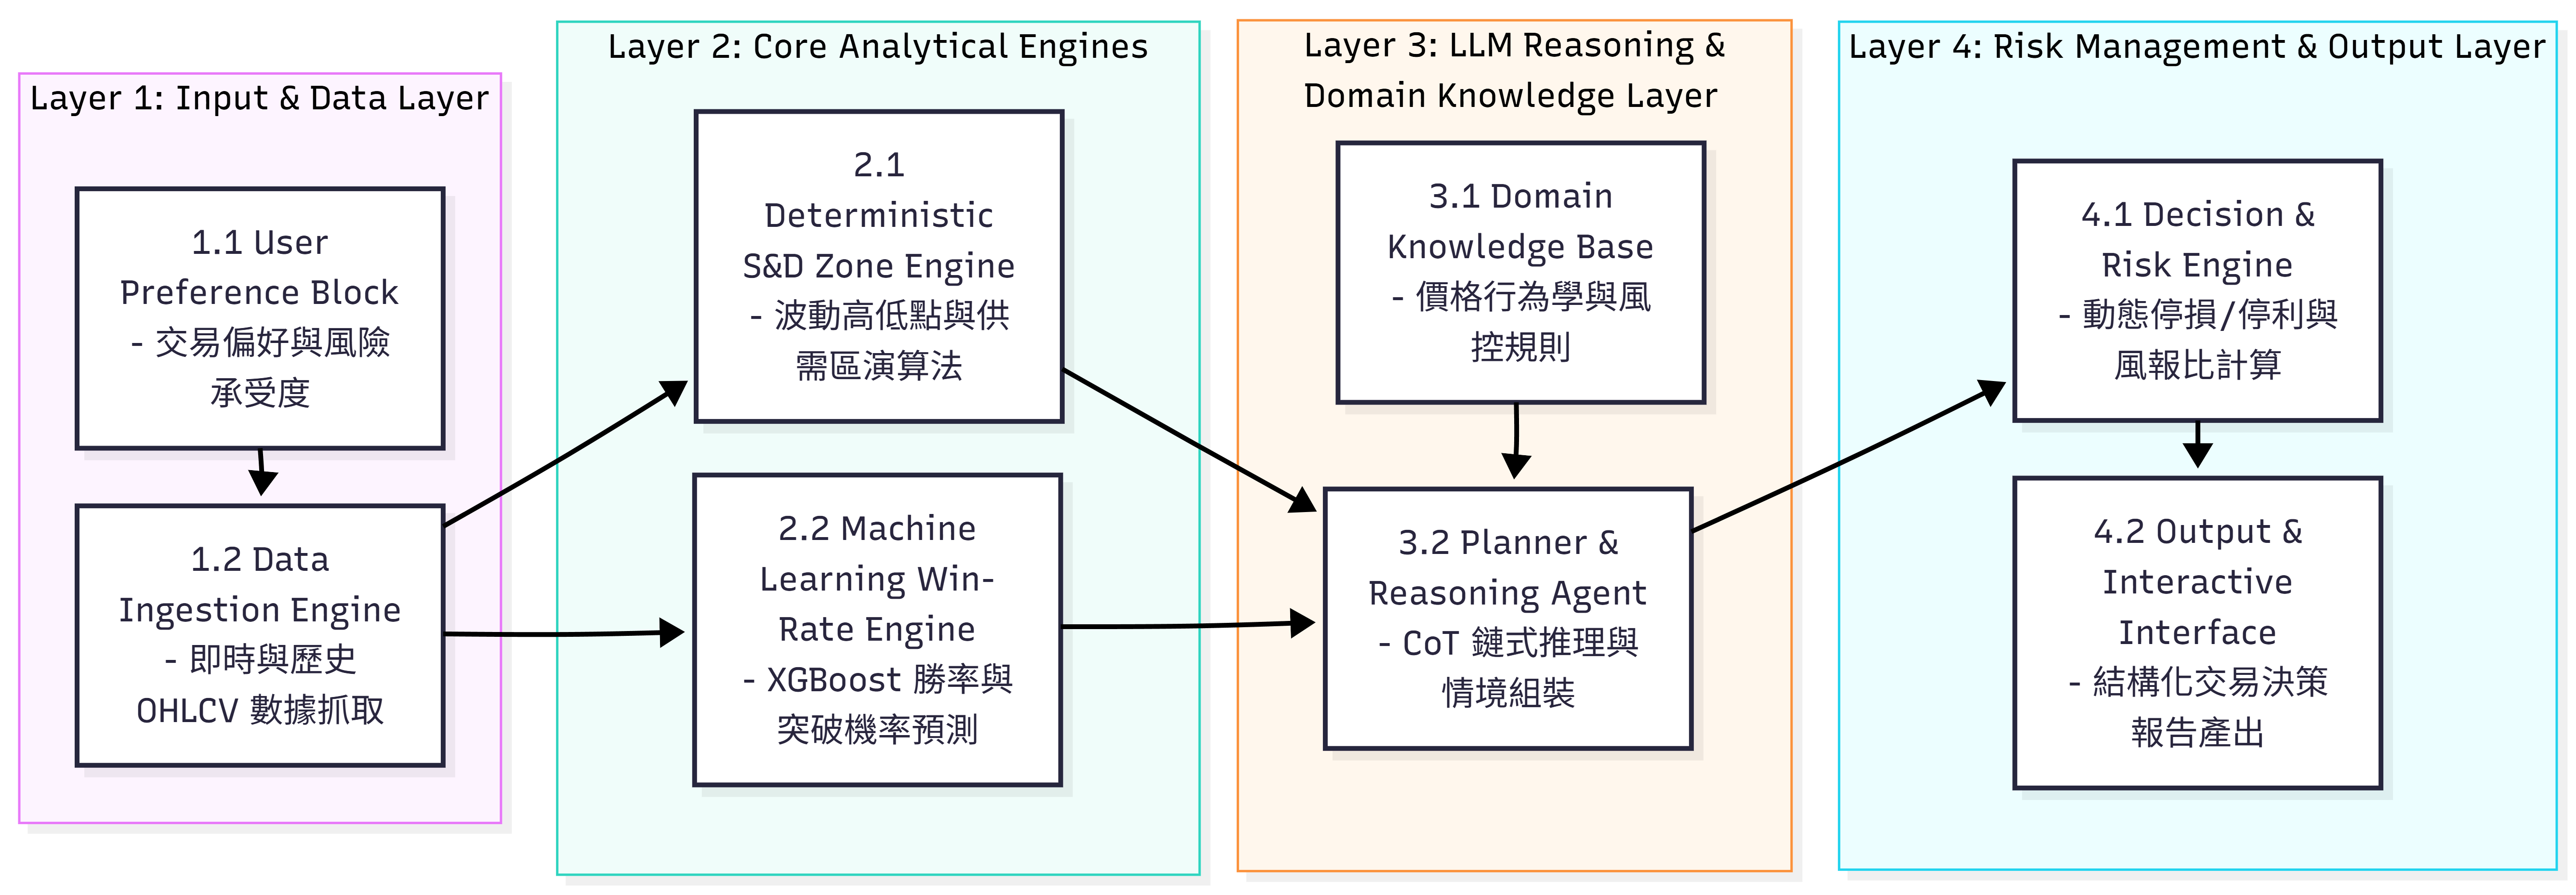
\includegraphics[width=\columnwidth]{fig1_arch.png}
\caption{Four-tier, eight-module decoupled architecture of Hybrid TPA-Agent.}
\label{fig:arch}
\end{figure}

\begin{figure}[t]
\centering
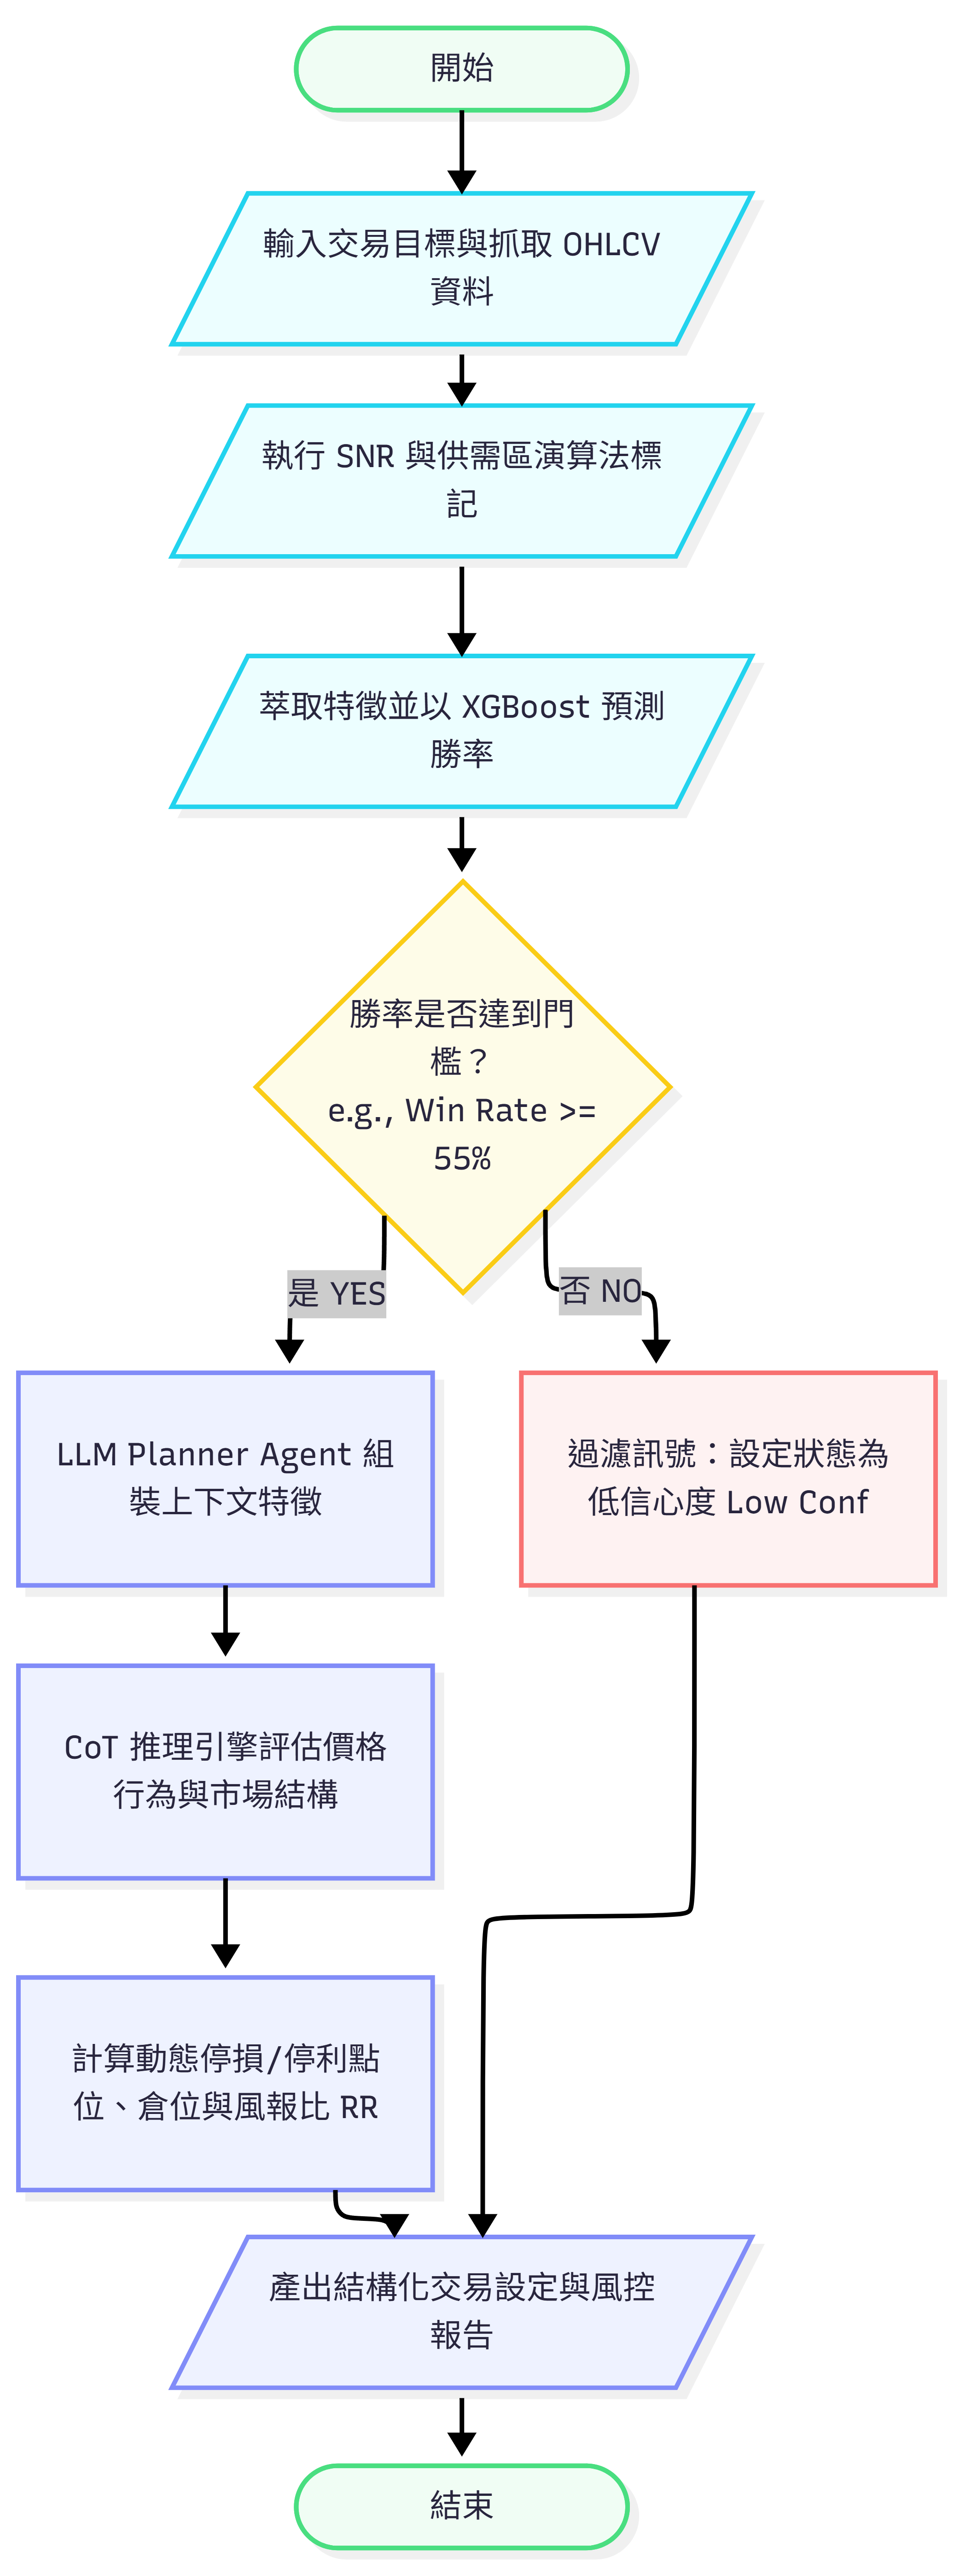
\includegraphics[height=0.38\textheight,keepaspectratio]{fig2_flow.png}
\caption{End-to-end decision and risk-gating execution flowchart.}
\label{fig:flow}
\end{figure}

% PF: Formulation
\subsection{Mathematical Formulation and Risk Gating}
For a long candidate setup, Module~4.1 deterministically computes geometric risk-to-reward $\mathrm{RR}$, unit-risk cost-adjusted expectancy $E_{\text{net}}$, and risk-bounded position size $\mathrm{Pos}$:
\begin{equation}
\label{eq:rr}
\mathrm{RR} = \frac{P_{\text{tp}} - P_{\text{entry}}}{P_{\text{entry}} - P_{\text{sl}}},
\end{equation}
\begin{equation}
\label{eq:exp}
E_{\text{net}} = W \cdot \mathrm{RR} - (1 - W) - c_{\mathrm{rt}},
\end{equation}
\begin{equation}
\label{eq:pos}
\mathrm{Pos} = \frac{\mathrm{Equity} \times R_{\text{tol}}}{|P_{\text{entry}} - P_{\text{sl}}|},
\end{equation}
where $c_{\mathrm{rt}} \ge 0$ denotes normalized round-trip exchange fees and slippage per unit risk $R = |P_{\text{entry}} - P_{\text{sl}}|$ (symmetric equations apply to short setups). Approval requires $\mathrm{RR} \ge \mathrm{RR}_{\min}$, $E_{\text{net}} > 0$, $\texttt{is\_valid\_setup} = \mathrm{true}$, and healthy feed status.

% PI: Implementation (Algorithm 1) & Degradation
\subsection{Implementation Pipeline (Algorithm 1) and Degradation}
Algorithm~\ref{alg:tpa} specifies the end-to-end pipeline within a total latency budget under $1.5$\,s per closed bar. To safeguard capital during API instability or flash crashes, Module~4.1 enforces three degradation tiers: \textbf{Level~1} (feed delay $>2$\,s or LLM schema/timeout fault) freezes new entries via \texttt{WAIT/NO\_TRADE}; \textbf{Level~2} verifies exchange server-side hard stop-loss orders on open positions and blocks scaling; and \textbf{Level~3} (feed outage $>30$\,s or OOD circuit breaker) issues urgent alerts and defensive flatten/hedge actions.

\begin{algorithm}[t]
\caption{Hybrid TPA-Agent Decision Pipeline}
\label{alg:tpa}
\begin{algorithmic}[1]
\REQUIRE Symbol $S$, Timeframe $\mathrm{TF}$, Decision Time $t$, Risk Tolerance $R_{\text{tol}}$
\ENSURE Decision Report $R_{\text{final}}$ (\texttt{APPROVED} or \texttt{WAIT/NO\_TRADE})
\STATE $D \leftarrow \text{Ingestion.fetch\_pit}(S, \mathrm{TF}, \text{close\_time} \le t)$
\IF{$\text{HeartbeatLatency} > 2\text{\,s}$ \OR $\text{FeedOutage} > 30\text{\,s}$}
    \RETURN $\text{Risk.degrade}(\texttt{"WAIT/NO\_TRADE"})$
\ENDIF
\STATE $Z_{\text{dem}}, Z_{\text{sup}} \leftarrow \text{SDZoneEngine.detect\_and\_update}(D)$
\STATE $P_{\text{cur}} \leftarrow D.\text{close}[-1]$
\STATE $\mathbf{x} \leftarrow \text{FeatureExtractor.extract}(D, Z_{\text{dem}}, Z_{\text{sup}})$
\STATE $W \leftarrow \text{CalibratedXGBoost.predict\_proba}(\mathbf{x})$
\IF{$W < W_{\min}$}
    \RETURN $\text{Out.wait}(\texttt{"Low W"})$
\ENDIF
\STATE $\text{ctx} \leftarrow \text{ReadOnlyJSON}(P_{\text{cur}}, Z_{\text{dem}}, Z_{\text{sup}}, W)$
\STATE $\text{res} \leftarrow \text{PlannerAgent.reason\_cot}(\text{ctx}, \text{DomainKB}, \text{temp}=0)$
\STATE $P_{\text{sl}}, P_{\text{tp}}, \mathrm{RR}, E_{\text{net}} \leftarrow \text{Risk.compute}(P_{\text{cur}}, Z_{\text{dem}}, Z_{\text{sup}}, W)$
\IF{$\text{res.valid\_schema}$ \AND $\text{res.is\_valid\_setup}$ \AND $\mathrm{RR} \ge \mathrm{RR}_{\min}$ \AND $E_{\text{net}} > 0$}
    \STATE $\mathrm{Pos} \leftarrow \text{Risk.calc\_size}(P_{\text{cur}}, P_{\text{sl}}, R_{\text{tol}})$
    \RETURN $\text{Out.ok}(P_{\text{cur}}, P_{\text{sl}}, P_{\text{tp}}, \mathrm{RR}, \mathrm{Pos})$
\ELSE
    \RETURN $\text{Out.wait}(\texttt{"RR/Struct Fail"})$
\ENDIF
\end{algorithmic}
\end{algorithm}

% PJ: Jump to an Example
\subsection{Illustrative End-to-End Walkthrough (BTC/USDT 15m)}
Consider a representative \texttt{BTC/USDT} 15m snapshot: Module~2.1 scans 200 closed bars at \$64,250 and identifies an unmitigated demand zone [\$63,800, \$64,000] backed by Volume Profile HVN alongside an overhead supply zone [\$65,200, \$65,500]. When price retests \$63,950 after sweeping \$63,850 with a Volume Z-score of $+2.3$ and a long lower wick, Module~2.2 outputs calibrated $W = 0.62 \ge 0.55$. Module~3.2 validates a \textit{Liquidity Sweep / Pinbar} setup against Module~3.1. Module~4.1 sets $P_{\text{entry}} = \$63{,}950$, $P_{\text{sl}} = \$63{,}750$ (\$200 risk), and $P_{\text{tp}} = \$65{,}150$ (\$1,200 reward), giving $\mathrm{RR} = 6.0 \ge 2.0$, gross unit expectancy $0.62(6.0)-0.38 = +3.34$, and positive $E_{\text{net}}$ after 0.04\% taker fees, yielding an \texttt{APPROVED} decision sized to 1\% account risk.

% PM: Math Proof | PK: Key Advantages | PL: Later Simulation Bridge
\subsection{Expectancy Bounds, Key Advantages, and Simulation Bridge}
\begin{proposition}[Cost-Adjusted Positive Expectancy and Bounded Loss]
\label{prop:expectancy}
Under deterministic gating in \eqref{eq:rr}--\eqref{eq:pos} with calibrated probability $W \in [0,1]$, round-trip cost ratio $c_{\mathrm{rt}} \ge 0$, and hard server-side stop-loss $P_{\text{sl}}$, any \texttt{APPROVED} setup guarantees: (i) strictly positive net expectancy if and only if $W > \frac{1 + c_{\mathrm{rt}}}{1 + \mathrm{RR}}$, and (ii) nominal stop-loss equity exposure bounded by $\mathrm{Pos} \cdot |P_{\text{entry}} - P_{\text{sl}}| = \mathrm{Equity} \cdot R_{\text{tol}}$ (excluding extreme gap slippage).
\end{proposition}
\begin{IEEEproof}
Expanding $E_{\text{net}} > 0$ in \eqref{eq:exp} gives $W(\mathrm{RR} + 1) - 1 - c_{\mathrm{rt}} > 0 \iff W > (1 + c_{\mathrm{rt}})/(1 + \mathrm{RR})$ since $\mathrm{RR} > 0$. Substituting \eqref{eq:pos} into nominal risk loss yields $\mathrm{Pos} \cdot |P_{\text{entry}} - P_{\text{sl}}| = \mathrm{Equity} \cdot R_{\text{tol}}$.
\end{IEEEproof}
Notice that for $\mathrm{RR}_{\min} = 2.0$ and negligible friction $c_{\mathrm{rt}} \to 0$, break-even requires $W > 1/3$, so the candidate threshold $W_{\min} = 0.55$ builds an explicit safety margin against calibration drift and fee friction. Collectively, these design choices (\textbf{PK}) eliminate LLM arithmetic hallucination, enforce verifiable risk bounds, and short-circuit low-quality noise before LLM invocation. Section~\ref{sec:experiment} next (\textbf{PL}) specifies the simulation protocol that empirically tests these parameters and hypotheses ($\mathrm{RQ1}$--$\mathrm{RQ5}$).

\section{Experiment}
\label{sec:experiment}

% Disclosure
\textit{Disclosure:} In accordance with research integrity and OpenSpec governance, no backtest results are fabricated prior to specification execution. This section defines the falsifiable experimental protocol for five research questions ($\mathrm{RQ1}$--$\mathrm{RQ5}$).

% Q: Quality & Quantity Metrics | R: Related Methods | S: Simulation Setup | T: Tuning Parameters
\subsection{Metrics, Baselines, Simulation Setup, and Parameter Tuning (Q--T)}
\textbf{Evaluation Metrics (Q):} Four metric families test $\mathrm{RQ1}$--$\mathrm{RQ5}$:
\begin{itemize}
    \item \textbf{Prediction Quality ($\mathrm{RQ1}$):} Precision, ROC-AUC, and Brier Score (probability calibration).
    \item \textbf{Trading Performance ($\mathrm{RQ1, RQ2}$):} Net Return, Profit Factor (PF), Sharpe Ratio, and Maximum Drawdown (MDD) net of fees and slippage.
    \item \textbf{Decision Reliability ($\mathrm{RQ3}$):} Multi-run Consistency Rate across repeated runs, Numerical Error Rate, and Risk Violation Rate.
    \item \textbf{Abstention Quality ($\mathrm{RQ4}$):} Trade Retention Rate and counterfactual post-rejection returns of \texttt{WAIT/NO\_TRADE} signals.
\end{itemize}

\textbf{Related Baselines (R):} Hybrid TPA-Agent will be compared against four controls under identical market snapshots: \textbf{B1} (EMA+RSI rules), \textbf{B2} (Pure XGBoost), \textbf{B3} (Pure LLM Agent), and \textbf{Ablation} (S\&D + XGBoost without LLM CoT).

\textbf{Simulation Setup (S):} Experiments use 5m and 15m historical OHLCV data for \texttt{BTC/USDT} and \texttt{ETH/USDT} (2023--2024 development/test window plus the October 2025 \$19B liquidation stress window) under unified capital, 0.04\% taker fees, and slippage. Four sequential stages enforce rigor: (1) chronological Train/Val/Test splitting; (2) strict PIT snapshot isolation ($\text{close\_time} \le t$); (3) extreme-event stress testing; and (4) hash-committed forward simulation.

\textbf{Parameter Tuning (T):} Rather than over-optimizing post hoc, candidate thresholds $W_{\min} = 0.55$, $\mathrm{RR}_{\min} = 2.0$, lookback length $N \in [200, 500]$, and Volume Profile bin resolution $B$ will be sensitivity-tested on validation splits alongside counterfactual rejected-signal distributions.

% U: Useful Expected Targets | V: Verify Effectiveness (RQ1-RQ5)
\subsection{Hypothesized Expected Targets and Effectiveness Verification (U--V)}
Table~\ref{tab:targets} states the \textit{hypothesized expected targets} (\textbf{U}) used as falsifiable benchmarks across repeated runs (reporting variance and worst-case distributions rather than cherry-picked curves). Effectiveness verification (\textbf{V}) maps directly to $\mathrm{RQ1}$--$\mathrm{RQ5}$: $\mathrm{RQ1}$ holds only if S\&D+XGBoost improves Brier Score, ROC-AUC, and net PF over B2; $\mathrm{RQ2}$ holds only if adding LLM CoT reduces false breakouts and raises risk-adjusted Sharpe/MDD over Ablation; $\mathrm{RQ3}$ requires $>95\%$ consistency and $0\%$ numerical/risk violations versus B3; $\mathrm{RQ4}$ requires avoided counterfactual losses on \texttt{WAIT} signals to outweigh missed winners; and $\mathrm{RQ5}$ tests whether gains survive PIT isolation, the October 2025 crash, and forward simulation.

\begin{table}[t]
\centering
\caption{Hypothesized Expected Targets (Not Verified Results) for Two-Year Backtest Comparison}
\label{tab:targets}
\scriptsize
\setlength{\tabcolsep}{3.5pt}
\begin{tabular}{p{2.2cm} c c c c c}
\toprule
\textbf{Model / Baseline} & \textbf{Win Rate} & \textbf{PF} & \textbf{Sharpe} & \textbf{MDD} & \textbf{Consistency} \\
\midrule
B1: EMA+RSI & $\sim$41.2\% & 1.18 & 0.74 & $-$28.5\% & 100\% \\
B2: Pure XGBoost & $\sim$52.8\% & 1.35 & 1.12 & $-$22.1\% & 100\% \\
B3: Pure LLM & $\sim$46.5\% & 1.22 & 0.85 & $-$34.2\% & $<$60\% \\
Ablation: S\&D+XGB & $\sim$55.4\% & 1.62 & 1.58 & $-$15.8\% & 100\% \\
\textbf{Hybrid TPA-Agent} & \textbf{$\sim$59.2\%} & \textbf{1.94} & \textbf{2.15} & \textbf{$\le -$12.0\%} & \textbf{$>$95\%} \\
\bottomrule
\end{tabular}
\end{table}

\section{Conclusion}
\label{sec:conclusion}

% W: What proposed | X: eXcel | Y: Yields | Z: Zen / Limitations & Future Work
\textbf{Summary and Strengths (W--X):} This paper proposed \textit{Hybrid TPA-Agent}, reframing short-term cryptocurrency trading AI from unconstrained price prediction to verifiable functional decoupling across deterministic S\&D/HVN geometry, calibrated XGBoost filtering, JSON-constrained Price Action CoT auditing, and programmatic risk enforcement. By separating arithmetic from LLM semantics and treating \texttt{WAIT/NO\_TRADE} and three-level outage degradation as first-class components, the architecture directly targets numerical hallucination, seed instability, and unmanaged tail risk.

\textbf{Expected Yields (Y):} Formalized under OpenSpec specifications, the proposed four-stage PIT protocol establishes a transparent benchmark to test whether decoupling achieves $>95\%$ decision consistency, $0\%$ risk-rule violations, improved net Profit Factor, and $\le 12\%$ maximum drawdown under realistic 0.04\% taker fees and slippage.

\textbf{Limitations and Future Work (Z):} Several external-validity boundaries remain: (1) SEBI's 87.7\% loss statistic derives from Indian equity derivatives and serves as behavioral motivation rather than an exact crypto loss rate; (2) TradingAgents variance \cite{koviazin2026} and FinForesight leakage results \cite{finforesight2026} were measured on equity/fundamental benchmarks and require re-verification on 5m/15m crypto bars; (3) Volume Profile HVNs degrade during thin-liquidity holiday periods; and (4) external LLM API latency or silent model updates can perturb reproducibility despite $\text{temperature}=0.0$. Future work will execute the full four-stage PIT backtest and hash-committed forward simulation; if empirical ablation shows that LLM CoT gains do not justify API latency and cost over the S\&D+XGBoost ablation, that negative boundary will be reported explicitly.

\begin{thebibliography}{9}

\bibitem{sebi2026}
Securities and Exchange Board of India (SEBI), Dept.\ of Economic and Policy Analysis, ``Trading Behaviour of Individual Traders in the Equity Derivatives Segment (FY25--FY26),'' Official Regulatory Study, Aug.\ 2026.

\bibitem{reuters2025}
Reuters, ``Crypto markets face severe liquidation event amid volatile trading conditions,'' Market Report (\$19B+ leveraged liquidations), Oct.\ 2025.

\bibitem{brooks2012}
A.~Brooks, \textit{Reading Price Charts Bar by Bar: The Technical Analysis of Price Action for the Serious Trader}. Hoboken, NJ, USA: John Wiley \& Sons, 2012.

\bibitem{chen2016}
T.~Chen and C.~Guestrin, ``XGBoost: A scalable tree boosting system,'' in \textit{Proc.\ 22nd ACM SIGKDD Int.\ Conf.\ Knowl.\ Discov.\ Data Mining (KDD)}, 2016, pp.\ 785--794.

\bibitem{arxiv2407}
``Cryptocurrency price forecasting using XGBoost regressor and technical indicators,'' \textit{arXiv preprint}, 2024, doi: 10.48550/arXiv.2407.11786.

\bibitem{koviazin2026}
A.~Koviazin, T.~Mudarisov, E.~Polyachenko, and R.~State, ``Reproducibility in the TradingAgents framework,'' in \textit{Proc.\ 2026 Int.\ Conf.\ Artif.\ Intell.\ Fintech (ICAIF '26)}, ACM, 2026, pp.\ 365--370, doi: 10.1145/3800973.3801029.

\bibitem{finforesight2026}
FinForesight Authors, ``FinForesight: Assessing information leakage and LLM financial prediction capabilities,'' \textit{arXiv preprint}, 2026.

\bibitem{almeida2023}
J.~Almeida and T.~C.~Gon\c{c}alves, ``Cryptocurrency market microstructure: a systematic literature review,'' \textit{Ann.\ Oper.\ Res.}, 2023, doi: 10.1007/s10479-023-05627-5.

\bibitem{fission2026openspec}
Fission AI, ``OpenSpec: Spec-driven development for AI coding assistants,'' GitHub Repository, 2026. [Online]. Available: \url{https://github.com/Fission-AI/OpenSpec}

\end{thebibliography}

\end{document}
